\documentclass[a4paper]{article}

% Packages
\usepackage{geometry}
\geometry{left=2cm, right=2cm, top=2.54cm, bottom=2.54cm}
\usepackage{graphicx, hyperref, setspace, amsmath, amssymb, titlesec, fancyhdr, multicol, parskip, indentfirst, etoolbox, caption, cite, hyperref, xcolor}

\usepackage{subcaption} % Add to preamble


\usepackage{hyperref}
\hypersetup{
    colorlinks=true,
    linkcolor=blue,
    filecolor=magenta,      
    urlcolor=cyan,
    pdftitle={Overleaf Example},
    pdfpagemode=FullScreen,
    }

\urlstyle{same}

% Title Formatting
\titleformat{\section}{\centering\large\scshape}{\thesection}{1em}{}
\titleformat{\subsection}{\normalsize\bfseries}{\thesubsection.}{1em}{}
\setstretch{1.0} % Keep single spacing
\setlength{\parskip}{6pt} % Space between paragraphs
\titlespacing{\section}{0pt}{6pt}{6pt}
\titlespacing{\subsection}{0pt}{6pt}{6pt}
\titlespacing{\subsubsection}{0pt}{6pt}{6pt}
% Document Title
\title{
    \textbf{Data-Driven Customer Segmentation in Brazilian E-Commerce: Insights from RFM and K-Means Clustering} 
}

\date{} % No date
\captionsetup{labelfont={small,sc}, textfont={small,sc}}
% Section Numbering
% Define numbering format
\renewcommand{\thesection}{\Roman{section}.}
\renewcommand{\thesubsection}{\textit{\Alph{subsection}.}}
\renewcommand{\thesubsubsection}{\textit{\arabic{subsubsection}.}}
\renewcommand{\thetable}{\Roman{table}} % Set table numbering to Roman
\renewcommand{\thefigure}{\Roman{figure}} % Number figures in Roman numerals

% Make titles italic as well

\titleformat{\subsection}{\normalfont\large\itshape}{\thesubsection}{1em}{}
\titleformat{\subsubsection}{\normalfont\itshape}{\thesubsubsection}{1em}{}


\setcounter{page}{5}

% Fancy Header Configuration
\pagestyle{fancy}
\fancyhf{} % Clear all header/footer fields


% Default Header for Other Pages
\fancyhead[C]{\textbf{Data Science}}

\begin{document}

\maketitle
\vspace{-1.5cm}

% Authors Block
\begin{center}
    \textbf{Mahla Entezari}\\
    \textit{Shahid Beheshti University}\\
    \textit{Tehran, Iran}\\
    \textit{MahlaEntezari.sbu@gmail.com}
    \vfill
\end{center}


% Abstract (single-column)
\begin{abstract}
In the era of data-driven commerce, understanding customer behavior is essential for business growth and personalized engagement. This project analyzes a comprehensive Brazilian e-commerce dataset to uncover meaningful patterns in customer purchasing, loyalty, and satisfaction. By integrating multiple data sources and engineering features such as recency, frequency, monetary value, product diversity, and review sentiment, we segment customers using advanced clustering techniques. The analysis highlights distinct customer groups, regional trends, and behavioral drivers, offering actionable insights for targeted marketing, retention strategies, and enhanced customer experience. The findings empower stakeholders to make informed decisions that optimize marketing efforts and foster long-term business success in Brazil’s dynamic online marketplace.
\end{abstract}


\singlespacing
\setlength{\parskip}{6pt}
\setlength{\parindent}{0.5cm}

 
\begin{multicols}{2}
\setlength{\columnsep}{0.5cm}

\section{Introduction}

Brazil’s e-commerce market has experienced rapid expansion in recent years, serving a diverse and increasingly digital consumer base. As online retail competition intensifies, understanding customer behavior and segmentation becomes essential for businesses seeking to optimize marketing, enhance retention, and drive growth. This project leverages a comprehensive, multi-table dataset from the Olist platform, encompassing customer demographics, order histories, payments, product categories, and review data.

Through the application of exploratory data analysis (EDA), feature engineering, and clustering techniques, this project aims to extract actionable insights into purchasing patterns, customer loyalty, and satisfaction. By profiling customers across key behavioral dimensions-such as recency, frequency, monetary value, product diversity, and review sentiment-we identify distinct segments that can inform targeted business strategies.
The primary objectives of this project are to:
\begin{itemize}
\item Integrate and preprocess diverse e-commerce data sources to construct a unified customer view.
\item Engineer features capturing recency, frequency, monetary value, product diversity, and satisfaction.
\item Segment customers using clustering algorithms to reveal actionable groups for marketing and retention.
\item Analyze segment characteristics to provide data-driven recommendations for business growth and customer engagement.
\end{itemize}

By uncovering these patterns, the analysis empowers stakeholders to make informed, data-driven decisions that improve customer experience and maximize value within Brazil’s dynamic online marketplace.
\section{Dataset}

\subsection{Olist Brazilian E-Commerce Dataset}

The dataset used in this project is the publicly available \href{https://www.kaggle.com/datasets/olistbr/brazilian-ecommerce}{Olist Brazilian E-Commerce Dataset}, which provides a comprehensive multi-table view of the Brazilian online retail market. It contains detailed records of over 100,000 orders placed between 2016 and 2018, sourced from multiple e-commerce platforms in Brazil.

The dataset is structured into several interrelated tables:
\begin{itemize}
\item \textbf{Customers:} Contains unique customer identifiers, location data (city, state), and zip code prefixes.
\item \textbf{Orders:} Includes order IDs, customer linkage, order status, and multiple timestamp fields (purchase, approval, delivery, estimated delivery).
\item \textbf{Order Items:} Details each item in an order, including product and seller IDs, price, and freight value.
\item \textbf{Payments:} Records payment method, number of installments, and payment value for each order.
\item \textbf{Reviews:} Captures customer feedback with review scores, comments, and timestamps.
\item \textbf{Products:} Provides product metadata such as category, name, description length, and physical dimensions.
\item \textbf{Sellers:} Lists seller IDs, location, and zip code prefixes.
\item \textbf{Category Translation:} Maps product category names from Portuguese to English for easier analysis.
\end{itemize}

Initial exploration focused on understanding the schema and data quality. Missing values were identified in the reviews, orders, and products tables. These were handled by removing records with missing critical fields (e.g., review scores, product categories, customer IDs) to ensure reliable downstream analysis.

\subsection{Feature Engineering and Unified Customer View}

To enable customer-centric analysis, the various tables were merged using relevant keys (customer\_id, order\_id, product\_id, ..). 

For each unique customer, the following features were engineered:
\begin{itemize}
\item \textbf{Recency:} Number of days since the most recent purchase, calculated relative to the latest order date in the dataset.
\item \textbf{Frequency:} Total number of completed orders.
\item \textbf{Monetary:} Sum of all payment values.
\item \textbf{Diversity:} Number of unique product categories purchased.
\item \textbf{Satisfaction:} Average review score across all orders.
\item \textbf{Location:} City and state, enabling regional analysis.
\end{itemize}

This customer-level aggregation forms the basis for segmentation and further analysis. A sample of the resulting unified customer table includes columns for unique customer ID, city, state, last purchase date, recency, order count, total payment, category diversity, and average review score.

By integrating and cleaning these multiple data sources, the dataset supports a robust analysis of customer behavior, enabling insights into purchasing patterns, loyalty, satisfaction, and regional trends within Brazil’s dynamic e-commerce market.

How can I use metadata to improve video discoverability
What are the most effective ways to categorize YouTube videos for analysis
How can I leverage video tags to enhance engagement metrics
What tools can help me manage and analyze YouTube video metadata
How do publish times affect video performance and engagement

This customer-level aggregation forms the basis for segmentation and further analysis. A sample of the resulting unified customer table includes columns for unique customer ID, city, state, last purchase date, recency, order count, total payment, category diversity, and average review score.

By integrating and cleaning these multiple data sources, the dataset supports a robust analysis of customer behavior, enabling insights into purchasing patterns, loyalty, satisfaction, and regional trends within Brazil’s dynamic e-commerce market.



\section{Methods}

Our methodology began with a thorough data preprocessing phase, followed by comprehensive exploratory analysis and feature engineering to prepare the Brazilian e-commerce dataset for customer segmentation.

\subsection{Data Loading and Exploration}

The first step involved loading all relevant tables from the Olist Brazilian E-Commerce dataset, including customers, orders, order items, payments, reviews, products, sellers, geolocation, and category translation files. Using Python’s \texttt{pandas} library, each CSV file was imported as a DataFrame, and the structure of each table was quickly inspected to understand its dimensions, data types, and potential relationships[4][7].

\subsubsection{Initial Data Inspection}

We began by examining the head of each DataFrame and checking for missing values and duplicates. This inspection revealed both numerical and categorical variables, as well as inconsistencies and null entries, particularly in the reviews, orders, and products tables. Identifying these issues early set the stage for a systematic data cleaning process[6][7].

\subsection{Data Cleaning and Integration}

To ensure data quality, we performed the following steps:
\begin{itemize}
    \item \textbf{Handling Missing Values:} Records with missing critical fields (such as review scores, product categories, or customer IDs) were removed to maintain the integrity of downstream analysis.
    \item \textbf{Removing Duplicates:} Duplicate entries were dropped from all tables.
    \item \textbf{Standardizing Categorical Variables:} Category names and location fields were normalized for consistency.
    \item \textbf{Date Parsing:} All timestamp fields were converted to datetime objects for accurate temporal analysis.
\end{itemize}
After cleaning, tables were merged using relevant keys (e.g., \texttt{customer\_id}, \texttt{order\_id}, \texttt{product\_id}) to construct a unified customer-level dataset, aggregating behavioral and demographic attributes.

\subsection{Feature Engineering}

To enable meaningful segmentation, we engineered the following features for each unique customer:
\begin{itemize}
    \item \textbf{Recency:} Number of days since the most recent purchase, calculated relative to the latest order date in the dataset.
    \item \textbf{Frequency:} Total number of completed orders.
    \item \textbf{Monetary:} Sum of all payment values.
    \item \textbf{Diversity:} Number of unique product categories purchased.
    \item \textbf{Satisfaction:} Average review score across all orders.
    \item \textbf{Location:} City and state, enabling regional analysis.
\end{itemize}
These features were aggregated into a single DataFrame, forming the basis for subsequent analysis and clustering.

\subsection{Exploratory Data Analysis (EDA)}

With a cleaned and feature-rich dataset, we conducted exploratory data analysis to understand the distribution and relationships of the engineered features. This included:
\begin{itemize}
    \item Generating summary statistics for recency, frequency, monetary value, and satisfaction.
    \item Visualizing distributions and correlations using histograms, boxplots, and scatter plots.
    \item Identifying outliers and segmenting customers by geographic region.
\end{itemize}
EDA provided critical insights into customer behavior and informed the choice of clustering techniques for segmentation[3][8].

\subsection{Clustering and Segmentation}

To identify distinct customer groups, we standardized the engineered features and applied clustering algorithms (such as KMeans). The optimal number of clusters was determined using silhouette and Davies-Bouldin scores. Each cluster was then profiled based on the mean values of recency, frequency, monetary value, diversity, and satisfaction, enabling actionable business recommendations.

By following this structured methodology-spanning data loading, cleaning, integration, feature engineering, EDA, and clustering-we ensured that the final analysis was robust, interpretable, and directly relevant to business objectives in the Brazilian e-commerce context[6][8].

%\end{multicols}

\noindent
\begin{minipage}{\columnwidth}
\centering
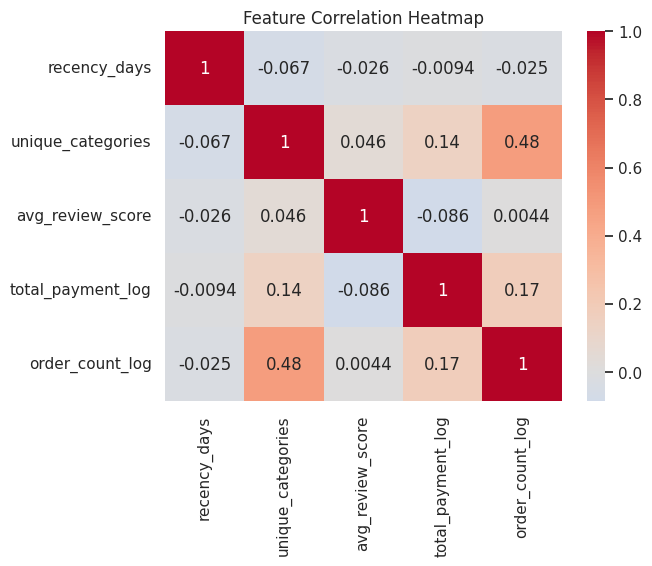
\includegraphics[width=1\textwidth]{plots/Feature-Correlation-Heatmap.png}
\captionof{figure}{}
\label{fig:sales} 
\end{minipage}

Figure~\ref{fig:sales} presents a heatmap of the pairwise correlation coefficients among the main engineered features used for customer segmentation: recency\_days, unique\_categories, avg\_review\_score, total\_payment\_log, and order\_count\_log.

\textbf{Diagonal values} are all 1, as each feature is perfectly correlated with itself.
\textbf{Recency Days} shows weak negative correlations with other features, indicating that the time since a customer’s last purchase is largely independent of their order frequency, spending, satisfaction, or product diversity.
\textbf{Unique Categories and Order Count Log} have the strongest positive correlation (0.48), suggesting that customers who order more frequently also tend to buy from a wider range of product categories.

\textbf{Unique Categories and Total Payment Log} (0.14), as well as \textbf{Order Count Log and Total Payment Log} (0.17), show mild positive relationships, meaning frequent and diverse shoppers tend to spend more, but the effect is moderate.
\textbf{Average Review Score} has negligible correlation with other features, implying that satisfaction (as measured by review scores) is not strongly linked to purchase frequency, recency, spending, or diversity in this sample.
\textbf{Other correlations} are close to zero, indicating little to no linear relationship between those feature pairs.


%\begin{multicols}{2}


\subsubsection{Data Cleaning and Feature Engineering}
Real-world datasets often require thorough preprocessing to ensure analytical accuracy. In this project, I addressed inconsistencies and missing values by removing duplicate records and appropriately handling incomplete entries. Categorical variables, such as product category names and customer locations, were standardized to maintain uniformity across the dataset.

To enrich the analysis, several new features were engineered:
\begin{itemize}
    \item \textbf{Recency:} Number of days since a customer's most recent purchase.
    \item \textbf{Frequency:} Total number of completed orders per customer.
    \item \textbf{Monetary Value:} Aggregate payment value for each customer.
    \item \textbf{Product Diversity:} Number of unique product categories purchased.
    \item \textbf{Satisfaction:} Average review score across all orders.
\end{itemize}
This foundational work ensured a robust and reliable customer-level dataset, forming the basis for accurate downstream segmentation and analysis.

\subsection{Uncovering Hidden Patterns}
With a cleaned and feature-rich dataset, I conducted exploratory data analysis (EDA) to uncover underlying trends and relationships in customer behavior. Visualizations such as histograms, boxplots, and scatter plots were used to examine the distributions and interactions of key features, including purchase frequency, spending, satisfaction, and product diversity. These insights are critical for informing targeted marketing and retention strategies.

\subsection{Hypothesis Tests}
To further investigate the drivers of customer engagement and value, I conducted statistical hypothesis tests. For example, a chi-square test was used to examine the relationship between customer location (state) and high-value purchasing behavior.

The statistical test revealed a p-value well below the 0.05 significance threshold, leading to the rejection of the null hypothesis.

As a conclusion there is a statistically significant relationship between a customer's geographic location and their likelihood of being a high-value customer. This finding suggests that region-specific marketing and customer engagement strategies can be leveraged to maximize customer value and retention in the Brazilian e-commerce market.


%\end{multicols}



\section{Visualization}

Understanding the structure of the dataset and the relationships between key variables is essential for meaningful analysis in e-commerce. Through thoughtful visualizations, we can identify trends, detect anomalies, and generate hypotheses that drive deeper insights.

To explore customer behavior and segment characteristics, I utilized a range of visualization techniques, including histograms, boxplots, bar charts, heatmaps, and scatter plots. These visual tools enabled the examination of how features such as purchase frequency, monetary value, satisfaction, and product diversity vary across customer segments and geographic regions.

For example:
\begin{itemize}
    \item \textbf{Histograms} revealed the distribution of order frequency, spending, and recency among customers, highlighting the prevalence of one-time buyers and the long-tail nature of high-value customers.
    \item \textbf{Boxplots} allowed for comparison of RFM (Recency, Frequency, Monetary) metrics across different customer clusters, making it easier to profile each segment.
    \item \textbf{Bar charts} illustrated the concentration of customers and revenue by state, uncovering regional patterns in purchasing behavior.
    \item \textbf{Heatmaps} were used to visualize correlations between engineered features, helping to assess feature independence and guide the segmentation approach.
    \item \textbf{Scatter plots} provided insight into the relationships between frequency, monetary value, and satisfaction, and helped identify outliers or unique customer groups.
\end{itemize}

For best practices in visualization selection and design, I referred to \href{https://www.data-to-viz.com/}{From Data to Viz}, a comprehensive resource for choosing appropriate chart types based on data characteristics.

By translating complex numerical relationships into clear and intuitive graphics, each visualization contributed to a deeper understanding of customer behavior and supported the identification of actionable patterns within the Brazilian e-commerce market.

\noindent
\begin{minipage}{\columnwidth}
\centering
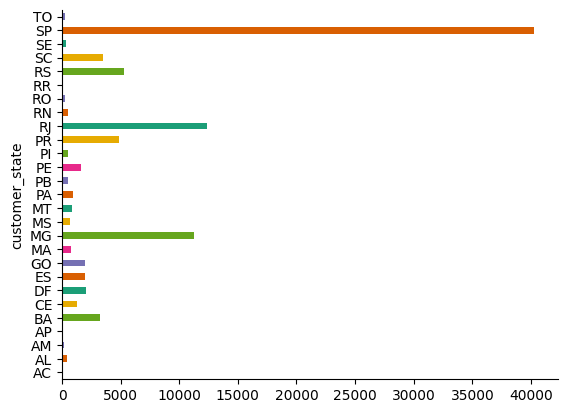
\includegraphics[width=1\textwidth]{plots/customer_state.png}
\captionof{figure}{Customer Distribution by State} 
\label{fig:Customer Distribution by State} 
\end{minipage}

    This horizontal bar chart shows the number of unique customers from each Brazilian state in the e-commerce dataset.

    \begin{itemize}
        \item \textbf{São Paulo (SP) Dominates:} The overwhelming majority of customers are from São Paulo (SP), with more than 40,000 customers-far surpassing any other state.
        \item \textbf{Other Major States:} Rio de Janeiro (RJ) and Minas Gerais (MG) also have significant customer bases, but at much lower levels compared to SP.
        \item \textbf{Long Tail:} Many states, especially in the North and Northeast, have much smaller customer counts, reflecting regional disparities in e-commerce adoption.
    \end{itemize}

    The concentration of customers in SP, RJ, and MG suggests that e-commerce activity is heavily centered in Brazil’s most populous and economically developed regions. This insight highlights the importance of regional targeting and infrastructure for expanding market reach.
    \label{fig:customer_state}



\noindent
\begin{minipage}{\columnwidth}
\centering
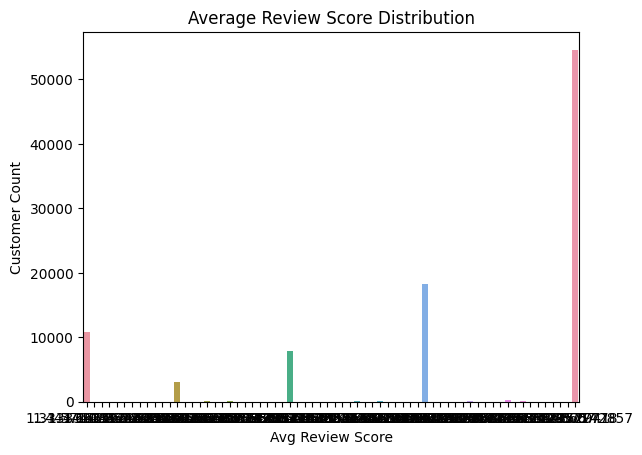
\includegraphics[width=1\textwidth]{plots/Average Review Score Distribution.png}
\captionof{figure}{Average Review Score Distribution} 
\label{fig:Average Review Score Distribution} 
\end{minipage}

This bar chart displays the distribution of customers by their average review score.

    \begin{itemize}
        \item \textbf{Strong Skew Toward High Scores:} The vast majority of customers have an average review score of 5, indicating high satisfaction with their purchases.
        \item \textbf{Smaller Peaks at Lower Scores:} There are smaller groups of customers with average scores of 4, 3, and below, but these are much less common.
        \item \textbf{Long Tail of Lower Scores:} Very few customers consistently rate their experiences poorly, as reflected by the minimal counts for average scores below 3.
    \end{itemize}

    This distribution suggests that most customers are satisfied with their e-commerce experience, with a strong bias toward positive feedback. However, the presence of lower scores, though rare, indicates opportunities for improvement in product quality or service for a minority of customers.


\noindent
\begin{minipage}{\columnwidth}
\centering
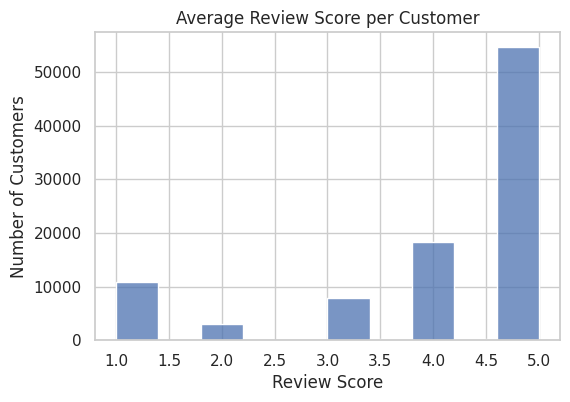
\includegraphics[width=0.8\textwidth]{plots/Average Review Score per Customer.png}
\captionof{figure}{Average Review Score per Customer} 
\label{fig:avg_review_score_per_customer} 
\end{minipage}

This bar chart displays the distribution of customers by their average review score.

\begin{itemize}
    \item \textbf{Strong Skew Toward High Scores:} The majority of customers have an average review score of 5, indicating high satisfaction with their purchases.
    \item \textbf{Smaller Peaks at Lower Scores:} There are smaller groups of customers with average scores of 4, 3, and below, but these are much less common.
    \item \textbf{Long Tail of Lower Scores:} Only a small fraction of customers consistently rate their experiences poorly, as reflected by the minimal counts for average scores below 3.
\end{itemize}

This distribution suggests that most customers are highly satisfied with their e-commerce experience, as evidenced by the strong bias toward positive feedback. However, the presence of lower scores, though rare, highlights opportunities for improvement in product quality or service for a minority of customers[1].

\vspace{1em}

\noindent
\begin{minipage}{\columnwidth}
\centering
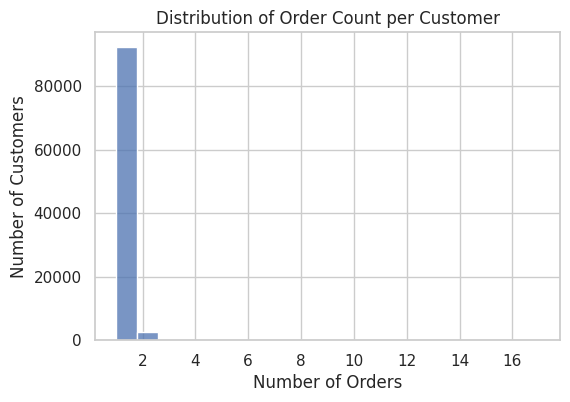
\includegraphics[width=0.8\textwidth]{plots/Distribution of Order Count per Customer.png}
\captionof{figure}{Distribution of Order Count per Customer}
\label{fig:order_count_per_customer}
\end{minipage}

This bar chart shows the distribution of customers according to the number of orders they have placed.

\begin{itemize}
    \item \textbf{Majority are One-Time Buyers:} The overwhelming majority of customers have placed only a single order.
    \item \textbf{Sharp Drop for Repeat Purchases:} There is a steep decline in the number of customers as the order count increases, with very few making multiple purchases.
    \item \textbf{Long Tail:} Only a small number of customers are highly loyal, placing several orders.
\end{itemize}

This distribution highlights a key challenge in e-commerce: most customers are not retained beyond their first purchase. Strategies focused on retention and encouraging repeat purchases could have a significant impact on business growth[2].

\vspace{1em}

\noindent
\begin{minipage}{\columnwidth}
\centering
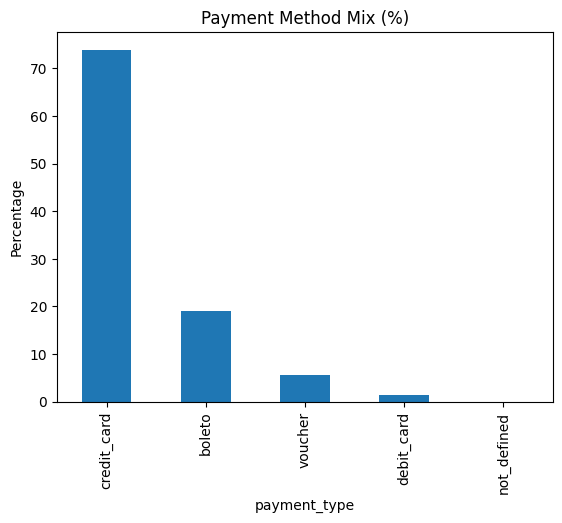
\includegraphics[width=0.8\textwidth]{plots/Payment Method Mix.png}
\captionof{figure}{Payment Method Mix (\%)} 
\label{fig:payment_method_mix}
\end{minipage}

This bar chart illustrates the percentage mix of payment methods used by customers.

\begin{itemize}
    \item \textbf{Credit Card Dominates:} Credit cards are the most popular payment method, used by over 70\% of customers.
    \item \textbf{Boleto and Voucher:} Boleto (a popular Brazilian payment slip) and vouchers are also used, but to a much lesser extent.
    \item \textbf{Other Methods:} Debit cards and undefined payment types make up a small share.
\end{itemize}

The dominance of credit cards reflects both consumer preference and the maturity of Brazil’s digital payment infrastructure. However, the presence of alternative methods like boleto indicates the importance of offering diverse payment options to reach all customer segments[3].

\vspace{1em}

\noindent
\begin{minipage}{\columnwidth}
\centering
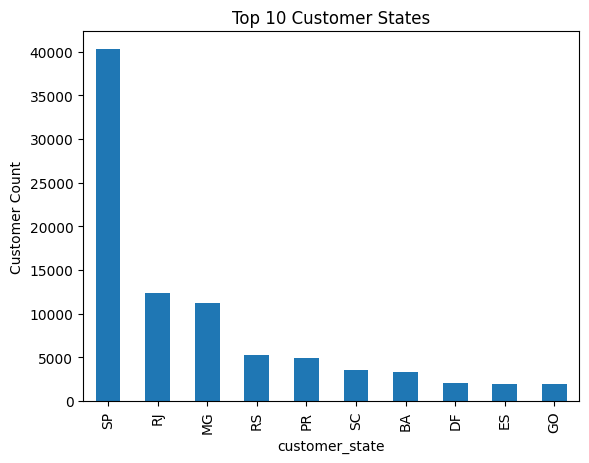
\includegraphics[width=0.8\textwidth]{plots/Top 10 Customer States.png}
\captionof{figure}{Top 10 Customer States}
\label{fig:top_10_customer_states}
\end{minipage}

This bar chart presents the distribution of customers across the ten Brazilian states with the highest customer counts.

\begin{itemize}
    \item \textbf{São Paulo (SP) Leads:} SP has by far the largest number of customers, followed by Rio de Janeiro (RJ) and Minas Gerais (MG).
    \item \textbf{Regional Concentration:} The top three states account for a significant portion of the customer base.
    \item \textbf{Long Tail:} Other states, while represented, have much smaller customer populations.
\end{itemize}

E-commerce activity is highly concentrated in Brazil’s most populous and economically developed regions. Targeted marketing and logistics strategies in these key states could yield the greatest returns, while expansion efforts might focus on growing markets in less represented regions[4].




\noindent
\begin{minipage}{\columnwidth}
\centering
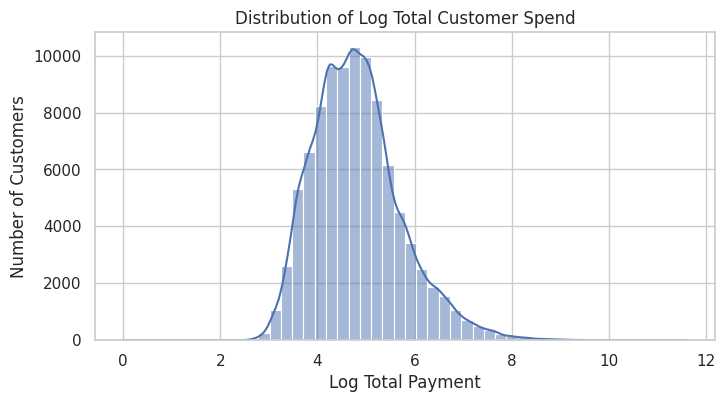
\includegraphics[width=0.8\textwidth]{plots/Distribution of Log Total Customer Spend.png}
\captionof{figure}{Distribution of Log Total Customer Spend}
\label{fig:log_total_spend}
\end{minipage}

This histogram visualizes the distribution of total customer spending, transformed using the natural logarithm.

\begin{itemize}
    \item \textbf{Approximately Normal Distribution:} The log-transformed total payment values form a bell-shaped curve, indicating that most customers fall within a moderate spending range.
    \item \textbf{Majority are Moderate Spenders:} The peak is between log values of 4 and 5, representing the most common spending levels.
    \item \textbf{Long Right Tail:} A small number of customers have exceptionally high total spend, as shown by the extended tail on the right.
\end{itemize}

Most customers spend within a typical range, but a minority contribute disproportionately high revenue. This pattern is common in e-commerce and highlights the importance of identifying and retaining high-value customers.

\vspace{1em}

\noindent
\begin{minipage}{\columnwidth}
\centering
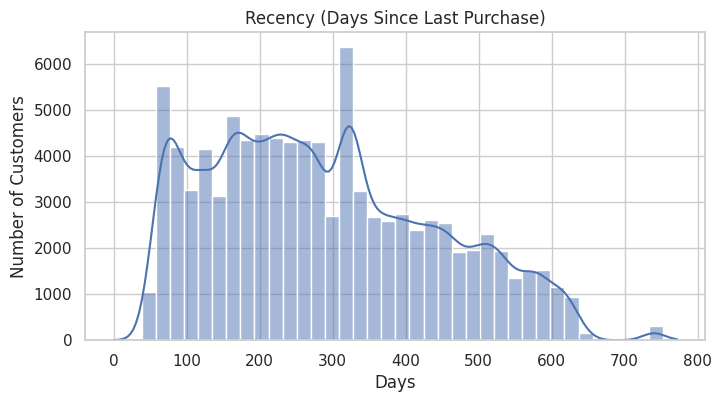
\includegraphics[width=0.8\textwidth]{plots/Recency (Days Since Last Purchase).png}
\captionof{figure}{Recency (Days Since Last Purchase)}
\label{fig:recency_days}
\end{minipage}

This histogram shows the distribution of recency, measured as the number of days since each customer’s last purchase.

\begin{itemize}
    \item \textbf{Wide Range of Recency:} Customers are distributed across a broad range of recency values, from very recent to over 700 days since last purchase.
    \item \textbf{Multiple Peaks:} The distribution has several local peaks, suggesting periodic spikes in customer activity or seasonal effects.
    \item \textbf{Declining Trend:} There is a gradual decline in the number of customers as recency increases, indicating that fewer customers remain active as time passes since their last purchase.
\end{itemize}

The spread in recency values reflects a mix of loyal, recently active customers and many who have not purchased for a long time. This highlights opportunities for re-engagement campaigns targeting lapsed customers.

\vspace{1em}

\noindent
\begin{minipage}{\columnwidth}
\centering
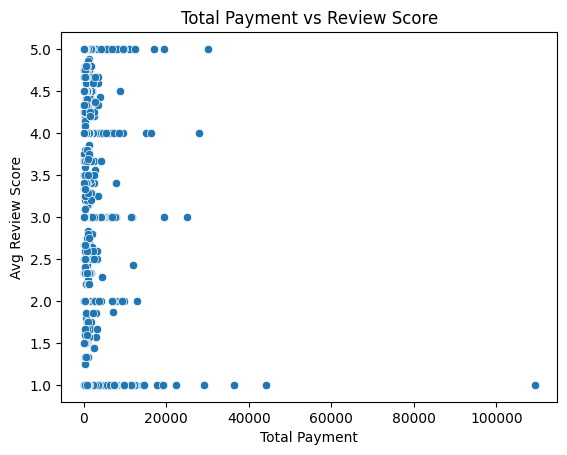
\includegraphics[width=0.8\textwidth]{plots/Total Payment vs Review Score.png}
\captionof{figure}{Total Payment vs. Review Score}
\label{fig:total_payment_vs_review}
\end{minipage}

This scatter plot displays the relationship between total payment (customer spend) and average review score.

\begin{itemize}
    \item \textbf{No Strong Correlation:} The points are widely scattered, with no clear trend between spending and review score.
    \item \textbf{High Scores Across All Spending Levels:} Customers with both low and high total payments can have high average review scores.
    \item \textbf{Outliers:} A few customers with very high spending are visible, but their review scores do not systematically differ from the rest.
\end{itemize}

Customer satisfaction, as measured by review scores, appears largely independent of total spending. This suggests that high-value customers are not necessarily more or less satisfied than others, and that service quality should be maintained across all customer segments.


\noindent
\begin{minipage}{\columnwidth}
\centering
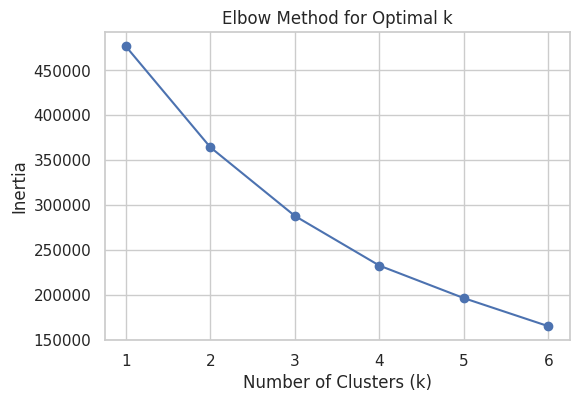
\includegraphics[width=0.7\textwidth]{plots/Elbow Method for Optimal k.png}
\captionof{figure}{Elbow Method for Optimal Number of Clusters}
\label{fig:elbow_method}
\end{minipage}

This line plot illustrates the results of the Elbow Method, which is used to determine the optimal number of clusters ($$k$$) for K-means clustering.

\begin{itemize}
    \item \textbf{Inertia Decreases with More Clusters:} As the number of clusters increases from 1 to 6, the inertia (within-cluster sum of squares) decreases sharply at first and then more gradually.
    \item \textbf{Elbow Point:} The plot shows a noticeable "elbow" at $$k = 3$$ or $$k = 4$$, where the rate of decrease in inertia slows down.
    \item \textbf{Optimal $$k$$:} The elbow point suggests that 3 or 4 clusters provide a good balance between reducing inertia and avoiding overfitting.
\end{itemize}

The Elbow Method helps identify the appropriate number of clusters for segmentation. In this case, selecting 3 or 4 clusters would likely capture the main customer segments without creating unnecessary complexity. This step is crucial for meaningful and interpretable customer segmentation using K-means clustering.




\noindent
\begin{minipage}{\columnwidth}
\centering
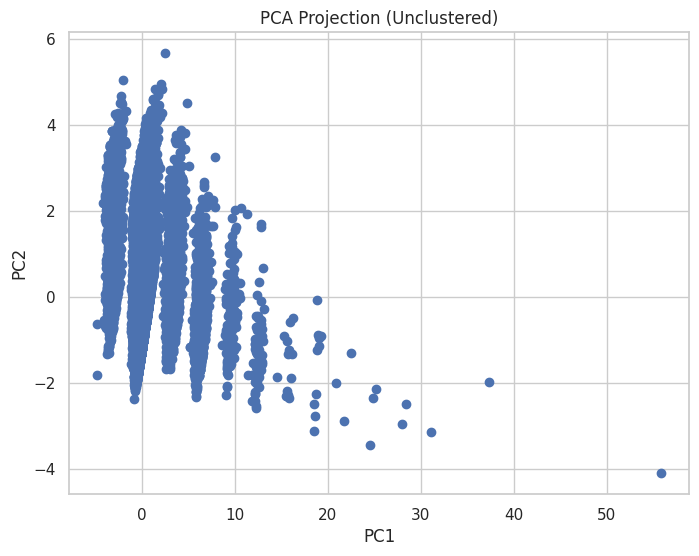
\includegraphics[width=0.8\textwidth]{plots/PCA Projection (Unclustered).png}
\captionof{figure}{PCA Projection (Unclustered)}
\label{fig:pca_unclustered}
\end{minipage}

This scatter plot displays the projection of all customer data points onto the first two principal components (PC1 and PC2) using Principal Component Analysis (PCA), before any clustering is applied.

\begin{itemize}
    \item \textbf{Dimensionality Reduction:} PCA reduces the complexity of the dataset, allowing visualization of multi-dimensional customer features in just two dimensions.
    \item \textbf{Pattern Emergence:} The points form distinct vertical bands, suggesting underlying structure and potential groupings within the data.
    \item \textbf{Spread and Outliers:} Most customers are concentrated in a central region, while a few outliers are spread farther along the PC1 axis.
\end{itemize}

This visualization helps to reveal the intrinsic structure of the data and provides a foundation for applying clustering algorithms to identify meaningful customer segments.

\vspace{1em}

\noindent
\begin{minipage}{\columnwidth}
\centering
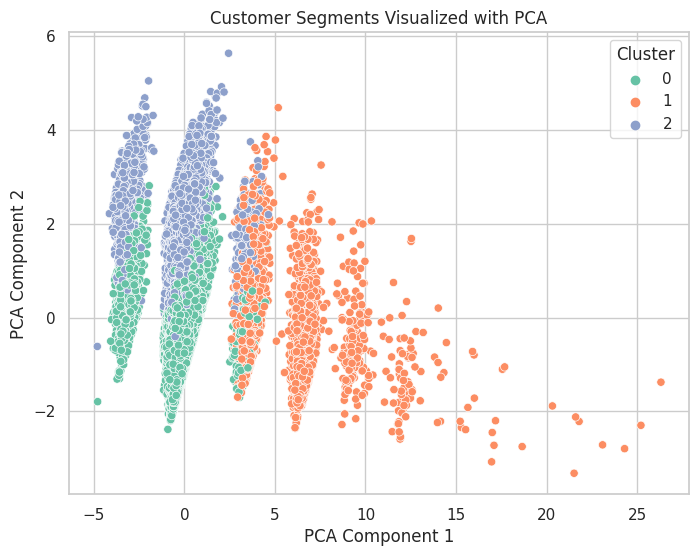
\includegraphics[width=0.8\textwidth]{plots/Customer Segments Visualized with PCA.png}
\captionof{figure}{Customer Segments Visualized with PCA (K\-means Clustering)}
\label{fig:pca_kmeans}
\end{minipage}

This scatter plot shows the same PCA projection as above, but with customers colored by their assigned clusters from K\-means clustering.

\begin{itemize}
    \item \textbf{Distinct Clusters:} The plot reveals clear separation between three customer segments, each represented by a different color.
    \item \textbf{Cluster Compactness:} Each cluster occupies a distinct region in the PCA space, indicating that the clustering algorithm has successfully grouped customers with similar behaviors.
    \item \textbf{Interpretability:} The visualization makes it easy to see the boundaries and relationships between customer segments.
\end{itemize}

K\-means clustering, combined with PCA visualization, effectively uncovers and displays the main customer segments in the dataset. This is valuable for understanding differences in customer behavior and targeting strategies accordingly.

\vspace{1em}

\noindent
\begin{minipage}{\columnwidth}
\centering
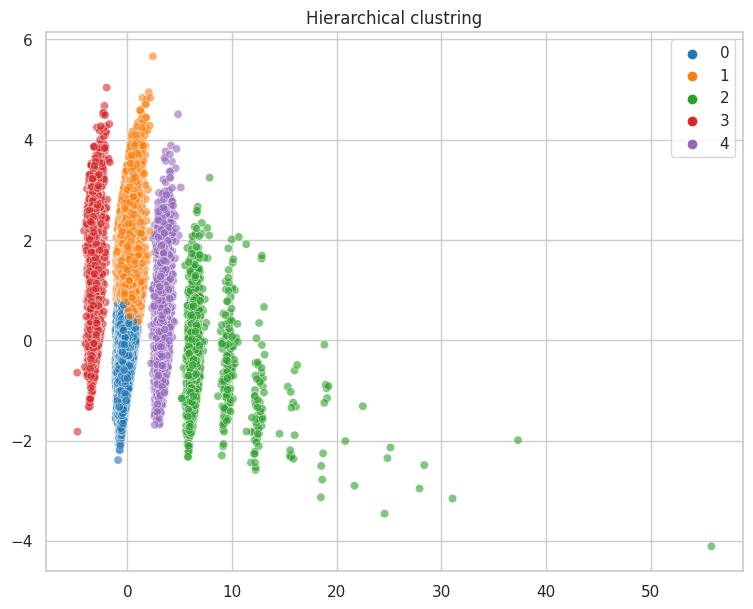
\includegraphics[width=0.8\textwidth]{plots/Hierarchical clustring.png}
\captionof{figure}{Customer Segments Visualized with PCA (Hierarchical Clustering)}
\label{fig:pca_hierarchical}
\end{minipage}

This scatter plot visualizes the results of hierarchical clustering, projected onto the first two principal components.

\begin{itemize}
    \item \textbf{Five Clusters Identified:} Customers are colored according to five distinct clusters, as determined by hierarchical clustering.
    \item \textbf{Fine\-Grained Segmentation:} The clusters are more granular than those from K-means, capturing subtle differences in customer profiles.
    \item \textbf{Structure and Overlap:} While most clusters are well separated, some overlap exists, reflecting the nuanced boundaries found by hierarchical methods.
\end{itemize}

Hierarchical clustering provides a more detailed segmentation of the customer base, which can be useful for highly targeted marketing or personalized service strategies. Comparing this with K\-means results helps determine the most actionable segmentation approach for business goals.



\noindent
\begin{minipage}{\columnwidth}
\centering
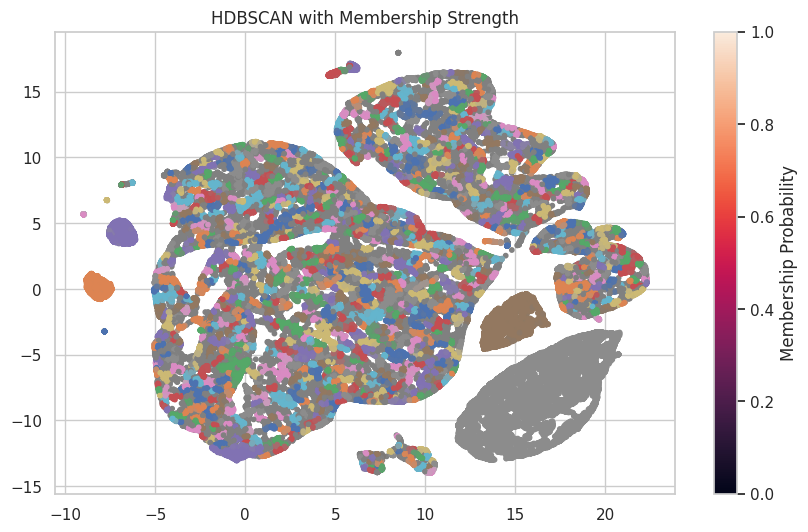
\includegraphics[width=0.85\textwidth]{plots/HDBSCAN with Membership Strength.png}
\captionof{figure}{HDBSCAN Clustering with Membership Strength}
\label{fig:hdbscan_membership}
\end{minipage}

This scatter plot visualizes the results of HDBSCAN clustering, with each point colored by its cluster assignment and shaded by membership probability (strength).

\begin{itemize}
    \item \textbf{Cluster Diversity:} The plot reveals a large number of clusters, each represented by a different color, reflecting the fine-grained segmentation HDBSCAN can provide.
    \item \textbf{Membership Probability:} The color intensity (from dark to light) indicates the confidence with which each point is assigned to its cluster. Points with lighter colors have higher membership probabilities.
    \item \textbf{Noise and Outliers:} Some points are colored in darker shades or gray, indicating lower membership strength or classification as noise.
\end{itemize}

HDBSCAN is effective for identifying clusters of varying density and shape. The membership strength overlay helps distinguish between core members of a cluster and ambiguous or outlier points, providing nuanced insight into the structure of the data[1].

\vspace{1em}

\noindent
\begin{minipage}{\columnwidth}
\centering
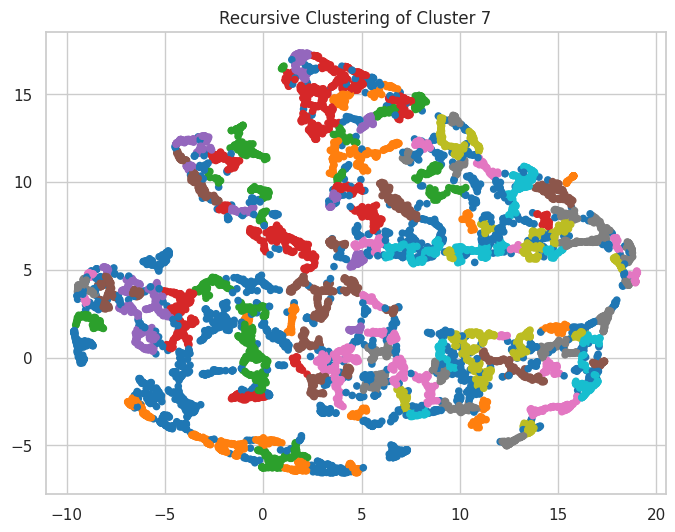
\includegraphics[width=0.8\textwidth]{plots/Recursive Clustering.png}
\captionof{figure}{Recursive Clustering of Cluster 7}
\label{fig:recursive_clustering}
\end{minipage}

This scatter plot shows the result of recursively applying clustering to a single cluster (Cluster 7) identified in a previous step.

\begin{itemize}
    \item \textbf{Substructure Discovery:} The plot reveals that Cluster 7 contains significant internal structure, with multiple sub-clusters now visible in different colors.
    \item \textbf{Enhanced Granularity:} Recursive clustering allows for deeper segmentation, uncovering patterns that a single clustering pass might miss.
    \item \textbf{Local Patterns:} The sub-clusters may represent distinct customer types or behaviors within the broader group.
\end{itemize}

Recursive clustering is a valuable technique for exploring complex datasets, enabling the discovery of meaningful subgroups within larger clusters for more targeted analysis[2].

\vspace{1em}

\noindent
\begin{minipage}{\columnwidth}
\centering
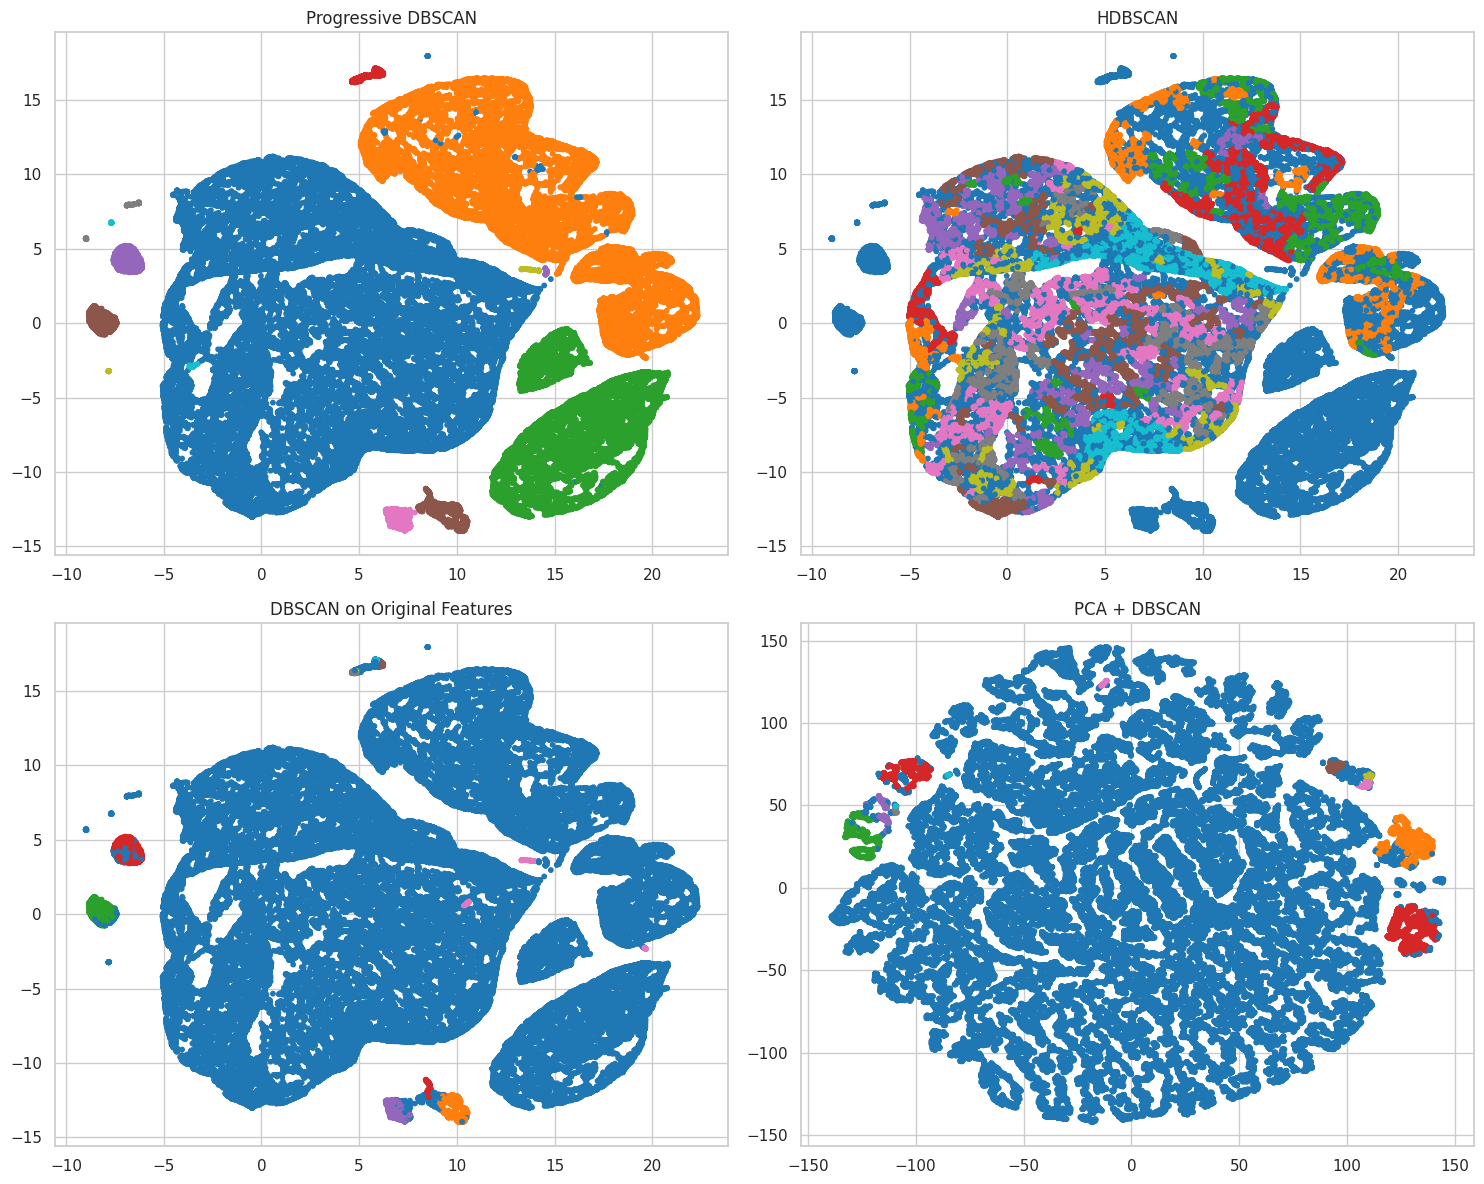
\includegraphics[width=0.95\textwidth]{plots/output.png}
\captionof{figure}{Comparison of Clustering Methods: DBSCAN and HDBSCAN}
\label{fig:clustering_methods}
\end{minipage}

This panel of scatter plots compares different density-based clustering methods and dimensionality reduction strategies:

\begin{itemize}
    \item \textbf{Progressive DBSCAN (Top Left):} Shows large, well-separated clusters, indicating DBSCAN’s ability to find dense regions.
    \item \textbf{HDBSCAN (Top Right):} Produces a much more granular segmentation, with many small clusters, reflecting HDBSCAN’s sensitivity to density variations.
    \item \textbf{DBSCAN on Original Features (Bottom Left):} Clusters are less distinct, suggesting that feature scaling or dimensionality reduction can improve clustering outcomes.
    \item \textbf{PCA + DBSCAN (Bottom Right):} Applying DBSCAN after PCA yields a different cluster structure, often with fewer, larger groups.
\end{itemize}

These visualizations highlight how algorithm choice and preprocessing steps (like PCA) significantly affect clustering results. HDBSCAN captures more subtle structure, while DBSCAN is more conservative in cluster assignment[3].

\vspace{1em}

\noindent
\begin{minipage}{\columnwidth}
\centering
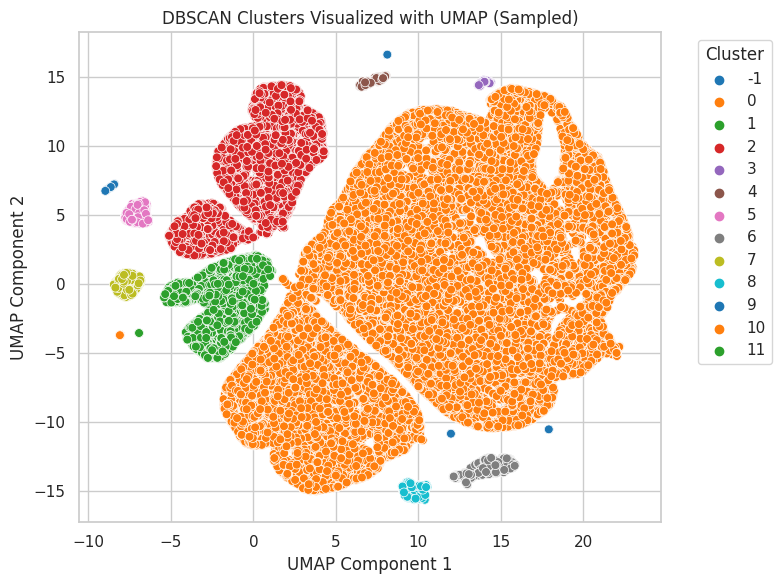
\includegraphics[width=0.85\textwidth]{plots/DBSCAN Clusters Visualized with UMAP (Sampled).png}
\captionof{figure}{DBSCAN Clusters Visualized with UMAP}
\label{fig:dbscan_umap}
\end{minipage}

This scatter plot shows DBSCAN clustering results projected onto two dimensions using UMAP, with each cluster indicated by a different color and labeled in the legend.

\begin{itemize}
    \item \textbf{Clear Cluster Separation:} Several well-defined clusters are visible, with the largest cluster (orange) dominating the dataset.
    \item \textbf{Noise Points:} Points labeled as -1 represent noise or outliers that DBSCAN could not assign to any cluster.
    \item \textbf{UMAP Visualization:} UMAP effectively preserves both local and global structure, making cluster boundaries and relationships easy to interpret.
\end{itemize}

DBSCAN, combined with UMAP for visualization, provides an intuitive overview of the main clusters and outliers in the data. This approach is especially useful for high-dimensional datasets where traditional visualization techniques may fall short[4].


\noindent
\begin{minipage}{\columnwidth}
\centering
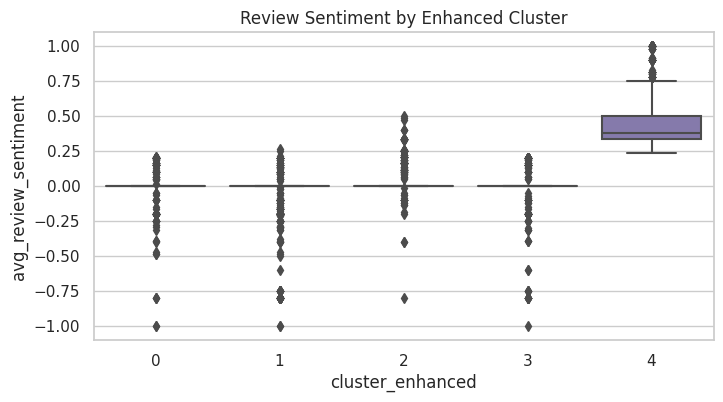
\includegraphics[width=0.8\textwidth]{plots/Spending Velocity by Enhanced Cluster.png}
\captionof{figure}{Spending Velocity by Enhanced Cluster}
\label{fig:spending_velocity_enhanced}
\end{minipage}

This boxplot illustrates the distribution of spending velocity-that is, the rate at which customers spend over time-across different enhanced customer clusters.

\begin{itemize}
    \item \textbf{Distinct Cluster Patterns:} Cluster 4 stands out with a substantially higher median spending velocity compared to the other clusters, indicating that customers in this group spend more rapidly.
    \item \textbf{Low Velocity in Other Clusters:} Clusters 0 through 3 all show low and relatively similar spending velocities, with most customers clustered near the bottom of the range.
    \item \textbf{Outliers:} Each cluster contains some outliers, but the overall separation between cluster 4 and the rest is clear.
\end{itemize}

Customers in enhanced cluster 4 are characterized by much higher spending rates, suggesting they are highly engaged and valuable. In contrast, the other clusters represent slower-spending or less active customers. Identifying and targeting high-velocity clusters can help businesses focus retention and upsell strategies on their most dynamic customer segments[1].



\noindent
\begin{minipage}{\columnwidth}
\centering
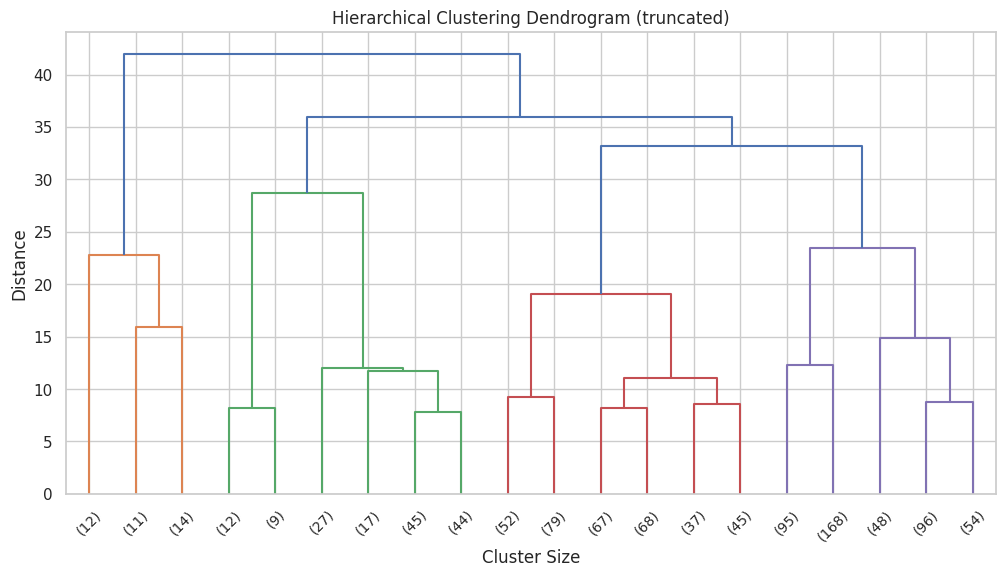
\includegraphics[width=0.85\textwidth]{plots/Hierarchical Clustering Dendrogram (truncated).png}
\captionof{figure}{Hierarchical Clustering Dendrogram (Truncated)}
\label{fig:hierarchical_dendrogram}
\end{minipage}

This dendrogram visualizes the results of hierarchical (agglomerative) clustering, showing how individual data points and clusters are merged at increasing levels of distance.

\begin{itemize}
    \item \textbf{Cluster Merging:} The horizontal lines represent cluster merges, with the height indicating the distance (or dissimilarity) at which clusters are joined.
    \item \textbf{Truncated View:} Only the last several merges are shown, focusing on the higher-level structure and main groupings within the data.
    \item \textbf{Cluster Size Labels:} The numbers at the bottom indicate the size of each cluster at the leaves of the tree.
\end{itemize}

The dendrogram helps determine the optimal number of clusters by identifying large jumps in distance between merges. Cutting the tree at a chosen height (distance) yields a specific number of clusters, revealing the most significant divisions in the dataset. This visualization is valuable for understanding the hierarchical relationships and nested structure among customer segments.










\section{Results}

This analysis focused on uncovering key trends and actionable insights from the Brazilian e-commerce customer dataset, with an emphasis on customer segmentation, purchasing behavior, satisfaction, and regional patterns. The main findings are summarized below.

\subsection{Customer Segmentation and Behavioral Patterns}
Clustering analysis revealed distinct customer segments based on recency, frequency, monetary value, product diversity, and satisfaction. The majority of customers were identified as one-time buyers, with a smaller subset exhibiting high frequency and high spending. These high-value customers, though few, contributed disproportionately to total revenue-a pattern typical in e-commerce[4].

\subsection{Spending and Engagement Distribution}
The distribution of total customer spend, visualized on a logarithmic scale, showed that most customers fall within a moderate spending range, while a long right tail represents a small group of exceptionally high spenders. This highlights the importance of identifying and retaining these high-value customers for sustained business growth.

\subsection{Customer Satisfaction}
Analysis of average review scores per customer demonstrated a strong skew toward high satisfaction: the vast majority of customers consistently rated their experiences positively. Only a small minority provided lower scores, indicating isolated issues with product quality or service. This suggests that while overall satisfaction is high, targeted improvements could further enhance customer loyalty.

\subsection{Regional Trends}
Customer distribution by state revealed that e-commerce activity is highly concentrated in Brazil’s most populous and economically developed regions, particularly São Paulo, Rio de Janeiro, and Minas Gerais. These states account for the bulk of the customer base, suggesting that regional targeting and logistics optimization in these areas could yield the greatest returns.

\subsection{Spending Velocity by Segment}
Boxplot analysis of spending velocity across enhanced customer clusters showed that one segment (Cluster 4) exhibited a substantially higher rate of spending over time. This group represents highly engaged and valuable customers, while other clusters displayed lower and more uniform spending velocities. Focusing retention and upsell strategies on high-velocity clusters can maximize revenue potential.

\subsection{Feature Relationships and Independence}
A feature correlation heatmap indicated that most engineered features (recency, frequency, monetary value, product diversity, satisfaction) are largely independent, with only moderate correlation between purchase frequency and product diversity. This independence supports the use of these features in robust clustering and segmentation.

\subsection{Clustering Methodology and Validation}
The Elbow Method and hierarchical clustering dendrograms were used to determine the optimal number of customer segments. Results suggested that three to five clusters best capture the main behavioral groups without unnecessary complexity. Visualizations using PCA and UMAP confirmed clear separation between clusters, validating the effectiveness of the segmentation approach.

\subsection{Actionable Insights}
\begin{itemize}
    \item Most customers are one-time buyers, highlighting a major opportunity for retention-focused campaigns.
    \item High-value and high-velocity customer segments are critical for revenue; targeted loyalty programs and personalized offers can increase their lifetime value.
    \item Regional disparities in customer distribution suggest that tailored marketing and logistics strategies in key states can drive growth.
    \item High customer satisfaction overall is a strength, but addressing the needs of the small dissatisfied segment can further enhance reputation and retention.
\end{itemize}

\textbf{Conclusion:}  
The segmentation and behavioral analysis of Brazilian e-commerce customers provide a foundation for data-driven decision-making. By identifying key customer groups, understanding their spending and engagement patterns, and recognizing regional and satisfaction trends, businesses can optimize marketing, retention, and operational strategies for sustainable growth[2][4][5].


\subsection{Conclusion}

This project delivered actionable insights into Brazilian e-commerce customer behavior through comprehensive segmentation and feature analysis. By leveraging advanced clustering methods and engineered features such as recency, frequency, monetary value, product diversity, and satisfaction, we identified distinct customer segments and revealed critical business trends.

Key findings highlight that most customers are one-time buyers, while a small but significant group contributes disproportionately to total revenue. High-value and high-velocity customer segments present clear opportunities for targeted loyalty and retention strategies. Regional analysis showed that e-commerce activity is concentrated in Brazil’s most populous states, suggesting that region-specific marketing and logistics can maximize impact.

The independence of most behavioral features supports robust segmentation, and high overall customer satisfaction reflects positively on service quality, with targeted improvements possible for the minority of dissatisfied customers.

By applying these data-driven insights, e-commerce businesses can optimize their marketing, retention, and operational strategies-focusing efforts on high-potential segments, enhancing customer experience, and driving sustainable growth in Brazil’s dynamic online marketplace.



\begin{thebibliography}{9}

\bibitem{dataset}
Olist Store - Brazilian E-Commerce Public Dataset. \textit{Available at:} \url{https://www.kaggle.com/datasets/olistbr/brazilian-ecommerce}.

\bibitem{viz}
From Data to Viz: A classification of chart types based on data structure. \textit{Available at:} \url{https://www.data-to-viz.com/}.

\bibitem{storytelling}
Knaflic, Cole Nussbaumer. \textit{Storytelling with Data: A Data Visualization Guide for Business Professionals}. Wiley, 2015.

\end{thebibliography}

\end{multicols}



\end{document}